\section{Zasada działania}
    
    \frame{\sectionpage}
    
    \begin{frame}{Założenia projektu}
        \begin{itemize}
            \item Zbieranie danych o temperaturze z wielu pomieszczeń
            \item Tworzenie akcji (if ... then ...)
            \item Integracja różnych urządzeń "inteligentnych"
        \end{itemize}
    \end{frame}
    
    \begin{frame}{Komunikacja urządzeń}
        \centering
        Urządzenia komunikują się za pomocą technologi wi-fi
        
\includegraphics[width = 0.5\textwidth]{images/3wifi.png}

    \end{frame}
    
    \begin{frame}{Odczyt temperatury}
        \centering
        Płytki NodeMCU odczytują dane z czujnika temperatury i wysyłają je za pomocą wifi do raspberry pi
        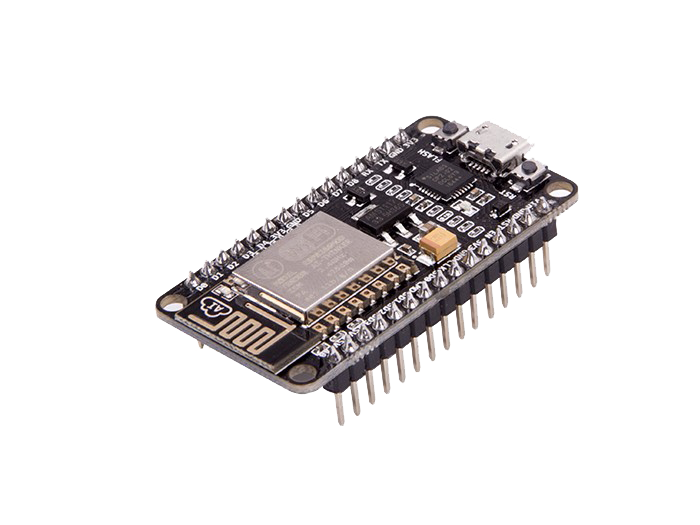
\includegraphics[width = 0.8\textwidth]{images/4no.png}
    \end{frame}
    
    \begin{frame}{IF... THEN...}
        \centering
        Raspberry pi włącza "inteligentne" urządzenie np. klimatyzacje jeśli temperatura będzie powyżej x°C
        
    \end{frame}
    
    \begin{frame}{Dostęp online}
        \centering
        Dostęp do temperatury w pomieszczeniach z dowolnego miejsca na świecie.
        
    \end{frame}
    